% ------------------------------------ %
% Copyright (C) 2020 Marvin Strangfeld %
% ------------------------------------ %
\documentclass[conference]{IEEEtran}

\usepackage{cite}
\usepackage{amsmath,amssymb,amsfonts}
\usepackage{algorithmic}
\usepackage{graphicx}
\usepackage{textcomp}
\usepackage{listings}
\usepackage{xcolor}
\usepackage[hidelinks]{hyperref}
\usepackage{cleveref}
\usepackage{float}

% TODO: Correctly align the caption with the listing frame
\usepackage{caption}
\DeclareCaptionFont{white}{\color{white}}
\DeclareCaptionFormat{listing}{\colorbox{darkgray}{\parbox{\dimexpr\linewidth-0.7em\relax}{#1#2#3}}}
\captionsetup[lstlisting]{format=listing,labelfont=white,textfont=white}

\definecolor{codegreen}{rgb}{0,0.6,0}
\definecolor{codegray}{rgb}{0.5,0.5,0.5}
\definecolor{codepurple}{rgb}{0.58,0,0.82}
\definecolor{backcolour}{rgb}{1,1,1}

\lstdefinestyle{mystyle}{
    backgroundcolor=\color{backcolour},
    commentstyle=\color{codegreen},
    keywordstyle=\color{magenta},
    numberstyle=\tiny\color{codegray},
    stringstyle=\color{codepurple},
    basicstyle=\ttfamily\footnotesize,
    breakatwhitespace=false,
    breaklines=true,
    captionpos=t,
    keepspaces=true,
    numbers=left,
    numbersep=5pt,
    showspaces=false,
    showstringspaces=false,
    showtabs=false,
    tabsize=2,
    frame=single,
    xleftmargin=2em,
    framexleftmargin=1.57em,
    framexrightmargin=-0.5em
}

\lstset{style=mystyle}
\renewcommand{\lstlistingname}{Code}
\Crefname{listing}{Code}{Codes}
\crefname{listing}{code}{codes}

\def\BibTeX{{\rm B\kern-.05em{\sc i\kern-.025em b}\kern-.08em
    T\kern-.1667em\lower.7ex\hbox{E}\kern-.125emX}}
\begin{document}

\title{Finding Concurrency Bugs in Production}

\author{\IEEEauthorblockN{Marvin Alexander Strangfeld}
\IEEEauthorblockA{
    \textit{RWTH Aachen University}\\
    marvin.strangfeld@rwth-aachen.de}
}

\maketitle

\begin{abstract}
% TODO: Why in production?
Today's computer architectures rely more and more on parallel computing.
Single core processors were widely replaced by multi-core architectures optimized to run processes and threads concurrently.
To utilize the full performance of a device, programmers need to write their software with a high degree of parallelism.
This introduces the potential for bugs that would not occur in sequential programs due to non-determinism of the order of execution.
For this purpose tools and languages have been developed to ease the creation of concurrency aware programs and help programmers find concurrency bugs.
In this paper we will evaluate the different tools and techniques that are available to find, reproduce and fix concurrency bugs from the viewpoint of how usable they are in a production environment.
\end{abstract}

\begin{IEEEkeywords}
    [Software Engineering]: Testing and Debugging
\end{IEEEkeywords}


% ------------------------------------ %
% ----------- INTRODUCTION ----------- %
% ------------------------------------ %
\section{Introduction}

\subsection{Heisenbugs}

\begin{quote}
``Everyone knows that debugging is twice as hard as writing a program in the first place. So if you're as clever as you can be when you write it, how will you ever debug it?'' --- Brian W. Kernighan\cite{kernighan1974elements}
\end{quote}

Writing concurrent programs can be very challenging.
Computational work gets distributed among different processes and threads that need to synchronize to be able to speed up execution time on multi-core architectures.
Due to this complexity it is no surprise that bugs that are correlated to concurrency and parallel program execution occur quite often.
These bugs are also the most difficult to debug because they are so complex in their nature and not easy to reproduce.~\cite{tu2019go}
This is because of the non-determinism that is introduced when multiple \emph{threads} or \emph{processes} are executed simultaneously.
In contrast to sequential programs that only run on one thread and process, concurrent programs have multiple paths of execution that are executed independently from each other.
The order these threads are executed is determined by the operating system's scheduler.
Because a programmer like the program itself can not predict what resources also need processing time on a machine, the choice of the schedule has to be handled as non-predictable and therefore non-deterministic.
But non-deterministic behavior also means that a bug that is only triggered when a certain pattern of thread executions appear can not be reliably reproduced without knowing the schedule it appeared.

In 1986 Jim Gray introduced the term ``Heisenbug'' for these kind of software failures.
He wrote:

\begin{quote}
``The assertion that most production software bugs are soft -- Heisenbugs that go away when you look at them -- is well known to systems programmers. Bohrbugs, like the Bohr atom, are solid, easily detected by standard techniques, and hence boring. But Heisenbugs may elude a bugcatcher for years of execution. Indeed, the bugcatcher may perturb the situation just enough to make the Heisenbug disappear. This is analogous to the Heisenberg Uncertainty Principle in Physics.''\cite{gray1986computers}
\end{quote}

The complexity and uncertainty of concurrency bugs is also the reason for many studies that examine how these bugs occur and explore different ways on how to detect, fix or even avoid them.
Thus, numerous tools and techniques have been developed that propose different solutions to the problem of concurrency bugs.

In this paper we will evaluate some of these and how they can be used to ease the process of debugging concurrent bugs.
The main focus is on detecting bugs efficiently in production, which means that developers should be able to fix bugs with a minimum amount of work and time.
Also, the occurrence of concurrency bugs should be reported immediately with minimal overhead of computational resources.

All code examples are written in Go which is a statically typed programming language developed by Google.
The reason we are using Go and not C/C++ or Java is the recent popularity of it for writing highly concurrent programs.
Popular open-source projects like \emph{Kubernetes}, \emph{Docker} or \emph{Prometheus} are all written in Go.
In the official documentation of Go it claims: ``Go is expressive, concise, clean, and efficient. Its concurrency mechanisms make it easy to write programs that get the most out of multicore and networked machines, while its novel type system enables flexible and modular program construction.''~\footnote{\url{https://golang.org/doc/}}
So, Go tries to tackle some of the problems that arise when writing concurrent software application by their design of language.
% TODO: How does Go want to archive this?
Although it encourages programmers to use concurrency by \emph{message passing}, it is also possible to make use of \emph{shared memory}, which gives the developer a lot of freedom to orchestrate the parallel execution of threads.
Projects written in Go also tend to have more concurrency than projects written in traditional programming languages such as C~\cite{tu2019go} what makes it even more important for developers to catch concurrency bugs effectively.

\subsection{Table of Contents}

\Cref{sct:taxonomy} will give a brief introduction on the different types of concurrency bugs and their causes.
\Cref{sct:dynamic} wil cover some techniques to dynamically find concurrency bugs and reliably reproduce them.
\Cref{sct:testing} will show different methods of concurrency-aware testing to detect concurrency bugs automatically by manipulating the thread scheduler.
And \Cref{sct:static} will finally cover how to detect concurrency bugs with static code analysis.

% ------------------------------------ %
% --- TAXONOMY OF CONCURRENCY BUGS --- %
% ------------------------------------ %
\section{Taxonomy of Concurrency Bugs}
\label{sct:taxonomy}

\begin{figure}
    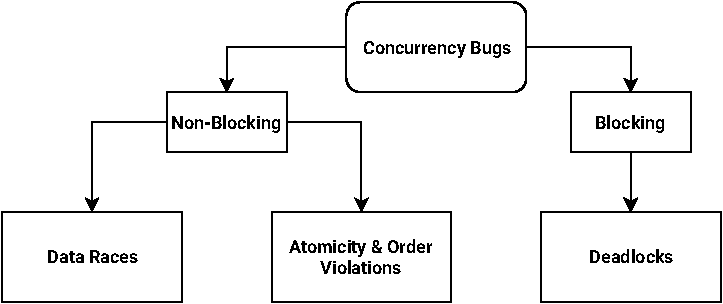
\includegraphics[width=\linewidth]{figures/ConcurrencyBugClasses.pdf}
    \caption{A Taxonomy of Concurrency Bugs -- based on\cite{tchamgoue2012testing}}
    \label{fig:classes}
\end{figure}

\Cref{fig:classes} shows a taxonomy of concurrency bugs based on the work of Tchamgoue, Kim and Jun.~\cite{tchamgoue2012testing}
For this paper we also distinguish between the two main categories of concurrency bugs: \emph{Blocking} and \emph{non-blocking}.
Blocking bugs are bugs where the execution of a program is unintentionally blocked and the program can not terminate.
The manifestation of these kind of bugs is very noticeable because the whole application freezes and has to be shutdown before the computation can continue.
Non-blocking bugs are often harder to find because they can occur even when the termination of a program was successful but the result is wrong.
This can also lead to a cascade of bugs where the root cause might not be obvious.

For example: A method might concurrently create a list of numbers that is expected to be ordered but due to a concurrency bug the list contains unordered elements.
This failure might only occur once in a thousand executions but if other methods depend on the correct order of elements in this list, the program might crash and the reason can be very hard to find.

\subsection{Deadlocks}
\begin{lstlisting}[float=h, language=Go, label=lst:deadlockWG, caption=Deadlock caused by waiting for the \emph{WaitGroup} at a wrong location -- based on \cite{tu2019go}]
func main() {
    var group sync.WaitGroup
    group.Add(len(data))
    for _, d := range data {
        go func(d string) {
            fmt.Printf("Processing: %s\n", d)
            defer group.Done()
        }(d)
        group.Wait() // Causing the bug
    }
}
\end{lstlisting}

\begin{lstlisting}[float, language=Go, label=lst:deadlockCh, caption={Deadlock caused by misuse of an \emph{unbuffered Channel}}]
func main() {
    ch := make(chan int)
    pr := make(chan int)
    ch <- 1 // Program already blocks here
    go func() {
        i := <-ch
        pr <- i
    }()
    <-pr
}
\end{lstlisting}

One example for blocking bugs are \emph{deadlocks} where circular dependencies between resources block the flow of a program.
\Cref{lst:deadlockWG} shows one example of such a deadlock in a Go program.
The problem is a \emph{blocking synchronization} where the \lstinline{group.Wait()} inside the for-loop is causing the block.

A second example of a deadlock that might not be obvious is \Cref{lst:deadlockCh} which uses two unbuffered channels to transfer information between threads.
The problem here is that without an active listener on an unbuffered channel any send action will be blocked.
To fix this one should use a buffered channel so the execution flow of the program can continue.

% TODO: Put this somewhere else
Another common problem in event-driven concurrent programs are \emph{blocking operations} like filesystem operations that are executed inside an event-handler.
These ``can penalize and even paralyze the entire program execution.''~\cite{tchamgoue2012testing}

\subsection{Data Races}
\begin{lstlisting}[float=h, language=Go, label=lst:race, caption=Data race -- based on \cite{goRaceDetector}]
func main() {
	c := make(chan bool)
	m := make(map[string]string)
	go func() {
		m["1"] = "a" // First conflicting access.
		c <- true
	}()
	m["2"] = "b" // Second conflicting access.
	<-c
}
\end{lstlisting}

Data races are part of the non-blocking concurrency bugs.
They occur when multiple threads simultaneously try to access a shared variable where at least one access is a write operation.~\cite{serebry2009threadsanitizer}

\Cref{lst:race} shows an example of a data race that is frequently found.~\cite{serebry2009threadsanitizer}
The data race happens when ``two threads access a non-thread-safe complex object [e.g. a map] without synchronization.''~\cite{serebry2009threadsanitizer}
Even though the two threads in this example write to different keys, this might cause a corruption of data or even crash the program.

\subsection{Atomicity and Order Violations}
\begin{lstlisting}[float=h, language=Go, label=lst:order, caption=Test-and-Use bug pattern -- Order violation]
func main() {
    data := getData()
    go func() {
        process(data)
        data = Nil
    }()
    if (data != Nil) {
        process(data) // Might already be Nil
    }
}
\end{lstlisting}

Atomicity and order violations are concurrency bugs where the interleaving of threads violate the programmer's intention of atomicity and order.
This often happens because:
``Most programmers think sequentially and therefore they make mistakes easily when writing concurrent programs.''~\cite{lu2008mistakes}

\Cref{lst:order} shows a common order violation bug pattern called ``Test-and-Use''.
The programmer's intention is to check if a variable is not Nil and then use this variable.
However, due to the thread that was launched before, it could happen that after the check in line 7, the thread of the goroutine gets scheduled and the data variable is set to Nil.

\begin{lstlisting}[float=h, language=Go, label=lst:atomicity, caption=Load-Store bug pattern -- Atomicity violation]
func main() {
    var group sync.WaitGroup
    group.Add(10)
    sum := 0
    for i = 0; i < 10; i++ {
        go func() {
            defer group.Done()
            sum++ // Not atomic
        }()
    }
    group.Wait()
}
\end{lstlisting}

\Cref{lst:atomicity} shows one example of the infamous ``Load-Store'' bug pattern.
The programmer assumes that ++ is an atomic operation because it is one literal in Go.
However, after compilation this is expanded to 3 instructions: LOAD, INCREMENT and finally STORE.
The thread scheduler could switch the context after any of these instructions what leads to undefined behavior.

Lu, Park, Seo and Zhou conducted a study in 2008 where they analyzed the characteristics of real-world concurrency bugs.~\cite{lu2008mistakes}
One key finding was that:
``Most of the examined non-deadlock concurrency bugs are covered by two simple patterns: atomicity-violation and order-violation''~\cite{lu2008mistakes}


% ------------------------------------ %
% ------ DYNAMIC CODE ANALYSIS ------- %
% ------------------------------------ %
\section{Dynamic Code Analysis}
\label{sct:dynamic}

One of the main techniques for finding concurrency bugs is dynamic code analysis.
In dynamic code analysis the runtime behavior of a program is observed to detect problematic patterns.

One popular implementation of this is ``Record and Replay'' where the path of execution of an application is recorded and can later be deterministically replayed.
This way programmers can easily find and fix those bug because, ``detecting concurrency bugs is difficult but once detected; correcting them is somehow an easy job.''~\cite{tchamgoue2012testing}
To create a recording that contains all information to replay a program exactly the same way it was executed, the recorder needs to keep track of the schedule of the program as well as all variables that might not be deterministically reproducible.
Like expected, this creates a lot of computational overhead in CPU time as well as storage.

To track the schedule of a natively compiled program such as Go programs, the record tool has to sit between the host operating system and the application.
One requirement to use such a tool in production is the ease of deployability which means that the operational overhead should be very small.
One example for a tool that fulfills this requirement is \emph{rr}~\footnote{\url{https://rr-project.org/}} developed by \emph{Mozilla}.
Their approach is to run the program on a fixed CPU core and track the system calls of the program by using \emph{\_ptrace\_}.
This way they can record programs on an unmodified Linux system and without compiling instrumentation into the programs code which might affect the concurrency behavior.
The main performance bottleneck are the context switches induced by ptrace.

Record and replay could therefore be a great tool to monitor applications in production.
Once a bug occurs and is either reported by a user or by the program itself, the programmer could just replay the thread schedule to reproduce, find and therefore fix the bug quickly.
Additionally, this technique can help to reproduce all kind of concurrency bugs no matter if they are blocking or non-blocking.
For programs that do not heavily depend on parallelism this approach is also very feasible.
The tool \emph{rr} can record such programs with a performance overhead below the factor of two.
However, for programs that heavily rely on parallelism the overhead to record and store the thread schedule can decrease the performance by more than a factor of 30.~\cite{o2017engineering}
Especially for multi-threaded server applications that expect a high workload and where speed is crucial for the business, this approach is not feasible in production, yet.
And even if the workload is low but the application is time-sensitive for example because of protocol timeouts, this technique is not applicable.

Another set of tools for dynamic code analysis are dynamic data race detectors.
As the name implies, these tools detect data races but because atomicity and order violations are often correlated, these tools can detect a variety of non-blocking concurrency bugs.
There are multiple approaches for data race detection but in this case we refer to on-the-fly and post-mortem data race detection which are often referred to as dynamic.~\cite{serebry2009threadsanitizer}
One data race detector that is mainly used for Go programs is the \emph{ThreadSanatizer} developed by Google.
% TODO: more about thread sanatizer performance

But ``data-race free does not mean concurrency bug free.''~\cite{lu2008mistakes}

% ------------------------------------ %
% ---- CONCURRENCY-AWARE TESTING ----- %
% ------------------------------------ %
\section{Concurrency-aware Testing}
\label{sct:testing}

Extensive testing has proven to minimize the bugs of software in production.\cite{makinen2014testing}
However, traditional testing mostly covers sequential errors and can not detect concurrency bugs effectively.\cite{lu2008mistakes}
This lies also in the nature of these bugs.
Only certain thread interleavings trigger the bug and therefore the tests could complete successfully almost every time without ever triggering the bug.
So new concurrency-aware tests are needed to find those bugs reliably.
One method of concurrency aware testing has been proposed by Choi and Zeller.\cite{acm2002}
% TODO: Reference for first occurrence of record and replay needed
They make use of a technique called ``Record and Replay'' that will be covered more in section \ref{sct:dynamic}

% ------------------------------------ %
% ------ STATIC CODE ANALYSIS -------- %
% ------------------------------------ %
\section{Static Code Analysis}
\label{sct:static}

Finally, static code analysis

% ------------------------------------ %
% ------------ CONCLUSION ------------ %
% ------------------------------------ %
\section{Conclusion}
\label{sct:conclusion}

Dynamic code analysis has the main disadvantage that it can cost a lot of overhead when monitoring is active in production.
Especially programs that heavily rely on multi-threaded execution like web-servers  can become very inefficient.

Static code analysis has the advantage that it can run independently from production servers for example inside a CI.
However, a high accuracy in detecting concurrency bugs requires a lot of computational resources due to the exponential growth of possible thread interleavings.

Concurrency-aware testing

\bibliographystyle{IEEEtran}
\bibliography{references}

\end{document}
